\documentclass{article}
\usepackage{ml1_homework_template}
\usepackage{amsmath}
\usepackage{amssymb}
% please submit the corresponding pdf by email to
% homework@class,brml.org, and write "homework sheet xx" in the 
% title.  No more, no less!  (Instead of xx, however,
% put the decimal number of the homework sheet.)

% Please update the following line, only change XX to the homework
% sheet number
\title{homework sheet 08}


\author{
\name{Andre Seitz}\\
\imat{03622870}\\
\email{andre.seitz@mytum.de}
\And
\name{Linda Leidig} \\
\imat{03608416}\\
\email{linda.leidig@tum.de}
}

% The \author macro works with any number of authors. There are two commands
% used to separate the names and addresses of multiple authors: \And and \AND.
%
% Using \And between authors leaves it to \LaTeX{} to determine where to break
% the lines. Using \AND forces a linebreak at that point. So, if \LaTeX{}
% puts 3 of 4 authors names on the first line, and the last on the second
% line, try using \AND instead of \And before the third author name.


\renewcommand{\Vec}[1]{\ensuremath{\mathbf{#1}}}
\newcommand{\Mtx}[1]{\ensuremath{\mathbf{#1}}}
\newcommand{\R}{\ensuremath{\mathbb{R}}}

\usepackage[numbered]{mcode}
\usepackage{graphicx}


\begin{document}
\maketitle

\section{Assignment: Covariance}
\paragraph*{Problem 1}
$\;$ 


\section{Assignment: Regression}
\paragraph*{Problem 2}
$\;$ 

We computed the values using Matlab. Here is the Matlab code:

\lstinputlisting{kernel.m}

\lstinputlisting{ex2.m}

For $l=1$ we get a mean value $\overline{y_*}$ of 0.3521 for both $x_*$.

The plots for different parameters $l$ follow on the next pages:

\begin{figure}[]
\centering
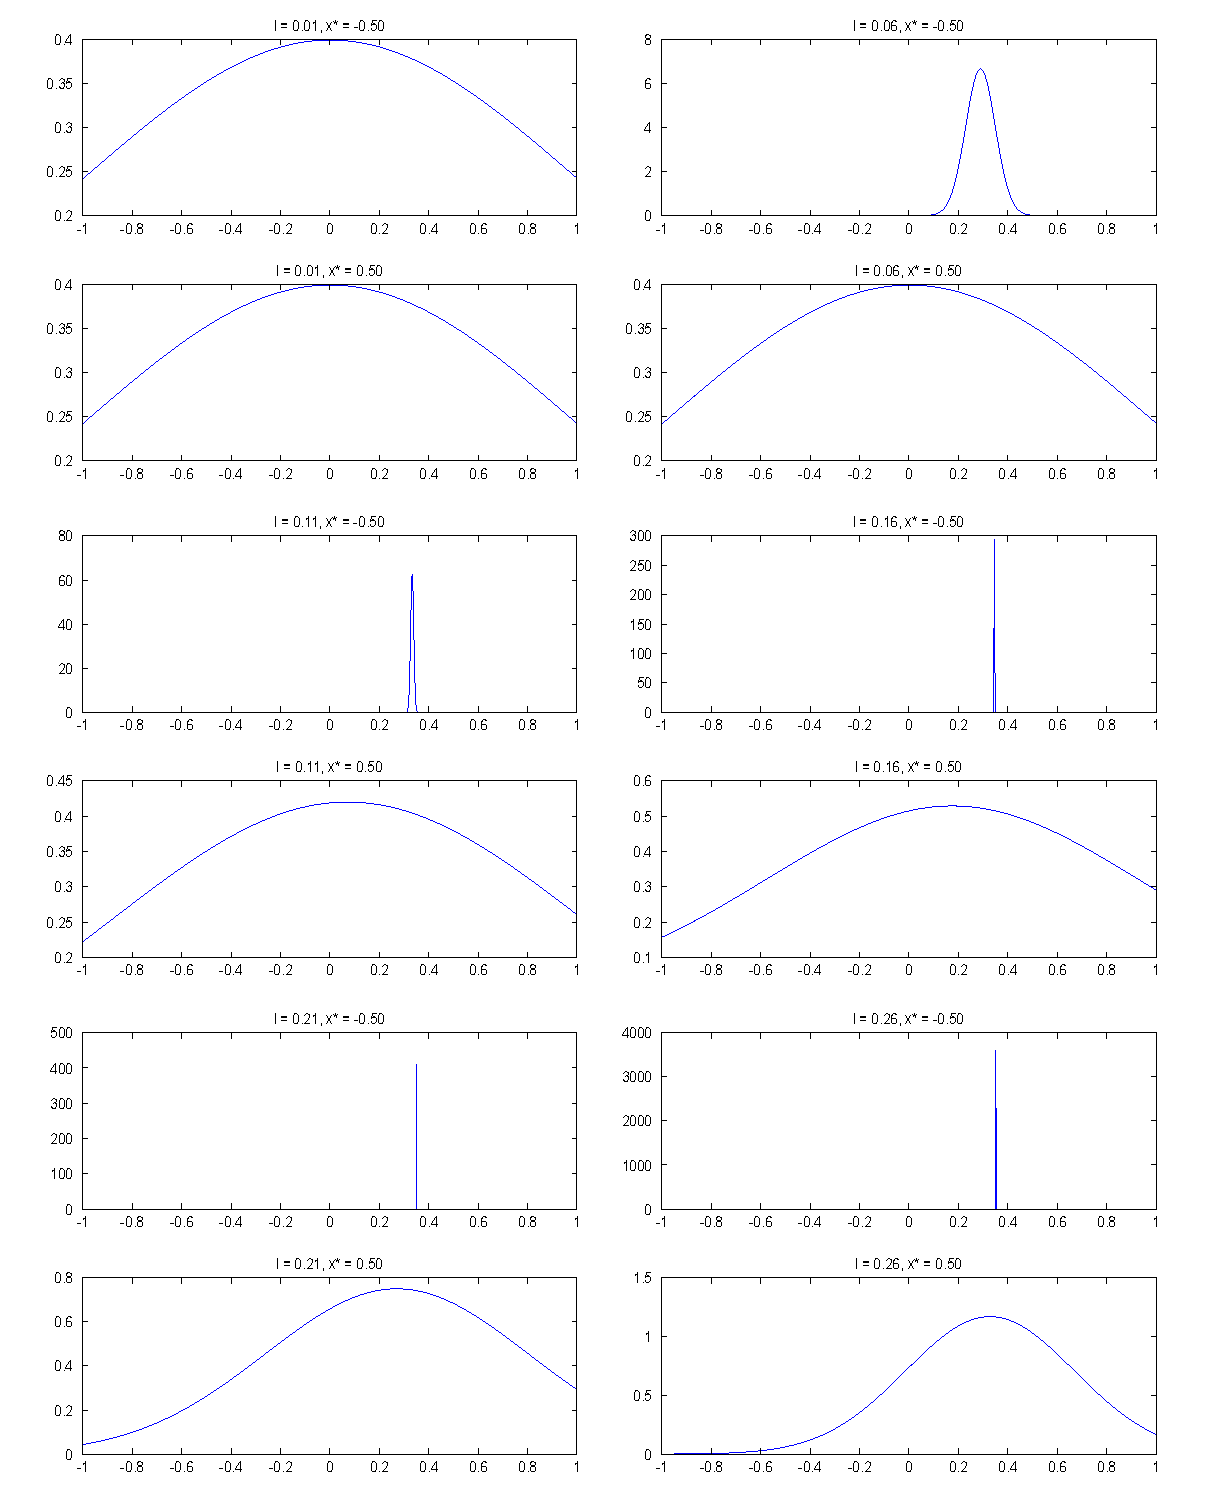
\includegraphics[width=\textwidth]{plots/page1.pdf}
\label{fig:mammary_structure}
\end{figure}

\begin{figure}[]
\centering
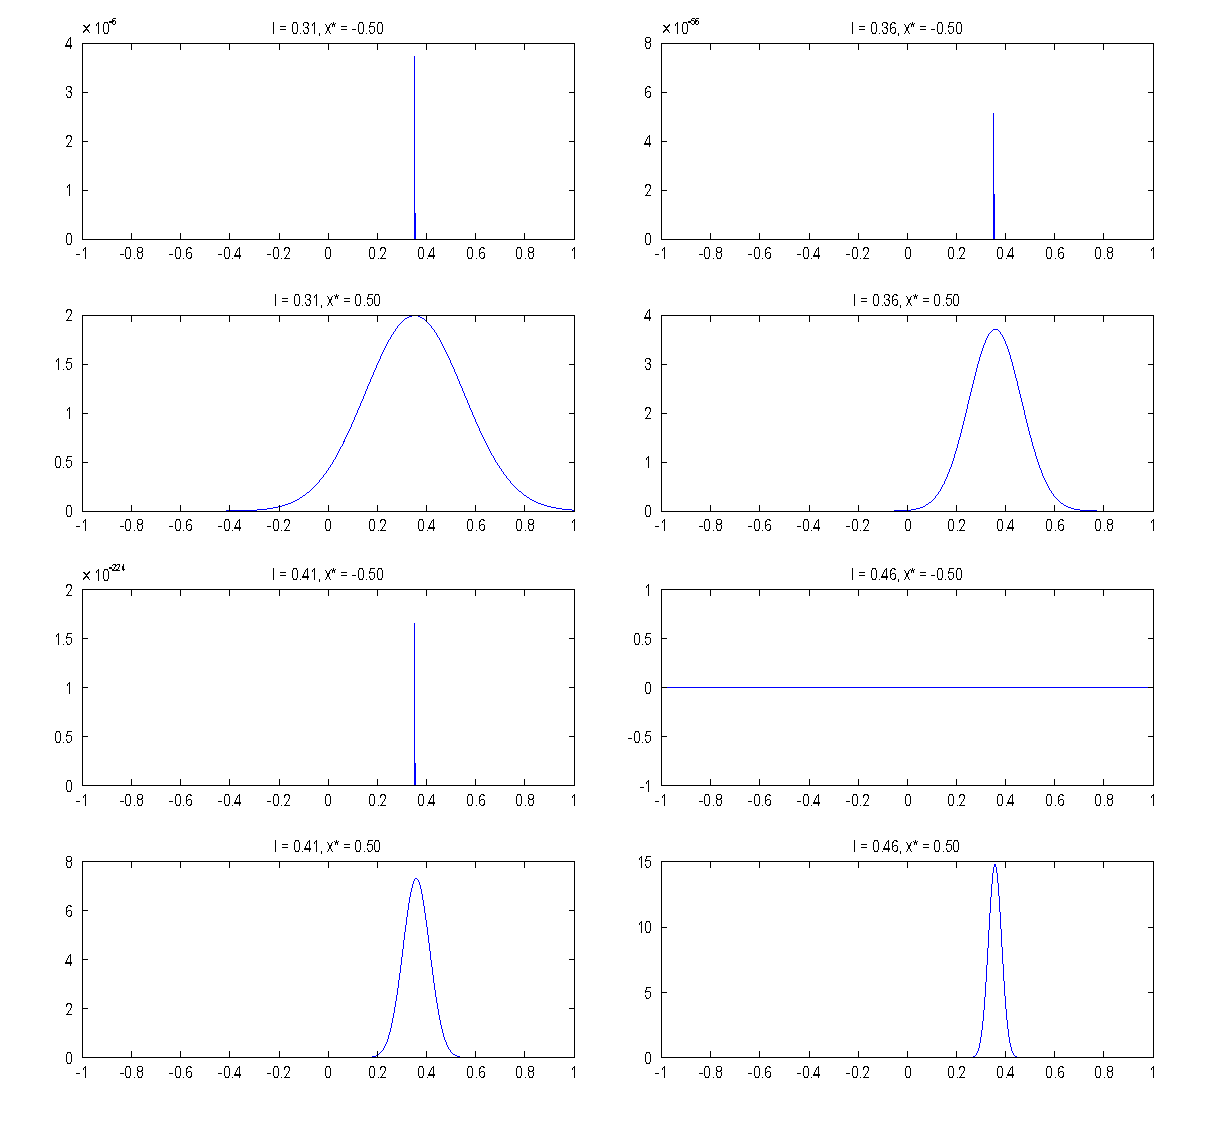
\includegraphics[width=\textwidth]{plots/page2.pdf}
\label{fig:mammary_structure}
\end{figure}


\end{document}
